\chapter{ Parsing Expression Grammars }
\label{ch:peg}

Οι δύο πιο συνηθισμένες μέθοδοι για να περιγραφεί η σύνταξη μίας γλώσσας σήμερα είναι οι κανονικές εκφράσεις και οι γραμματικές χωρίς συμφραζόμενα. 
Αυτοί οι φορμαλισμοί, ωστόσο, δεν είναι σε καμία περίπτωση ο μοναδικός τρόπος ορισμούς της συντακτικής δομής μίας γλώσσας. 
Ένα ακόμη χρήσιμο πρότυπο περιγραφής της σύνταξης είναι οι  \textit{Parsing Expression Grammars (PEGs)} \cite{Ford2004}, οι οποίες μοιάζουν με τις γραμματικές χωρίς συμφραζόμενα, αλλά έχουν και ορισμένες θεμελιώδεις διαφορές. 
Δαισθητικά, μια γραμματική χωρίς συμφραζόμενα μας περιγράφει το πώς  \textit{κατασκευάζεται} μία συμβολοσειρά που ανήκει σε κάποια γλώσσα, ενώ οι  PEGs  το πώς  \textit{αναλύεται} η συμβολοσειρά ώστε να προκύψει δομική πληροφορία για αυτή - εξ ου και το όνομα  "parsing language". 

Δεδομένου ότι η περιγραφή των γλωσσών (συνήθως) γράφεται από ανθρώπους και διαβάζεται από μηχανές, οι  Parsing Expression Grammars αποτελούν διαισθητικά ένα πιο κατάλληλο εργαλείο προσδιορισμού 
από τις γραμματικές χωρίς συμφραζόμενα. 
Ο σχεδιαστής της γραμματικής είναι ευκολότερο να σκέφτεται πώς αναλύεται μία δοσμένη συμβολοσειρά στα συστατικά της, παρά πώς θα γεννηθεί (generated) η συμβολοσειρά μέσα από τους κανόνες της γραμματικής.
% TODO: example to prove aforementioned claim

Πολλά συντακτικά ιδιώματα των σύγχρονων γλωσσών προγραμματισμού εκφράζονται ευκολότερα και πιο "φυσικά" σε  Parsing Expression Grammars. 
Επιπρόσθετα, οι PEGs μπορούν να αναλυθούν συντακτικά σε γραμμικό χρόνο, χρησιμοποιώντας το  Packrat Parsing  που περιγράφεται σε επόμενη ενότητα, την ώρα που μόνο μία συγκεκριμένη υποκλάση των γλωσσών χωρίς συμφραζόμενα μπορεί να αναλυθεί σε γραμμμικό χρόνο.

\section{Ορισμός των  Parsing Expression Grammars}
 Όπως με τις  Context Free,  οι  Parsing Expression Grammars χρησιμοποιούν τόσο τερματικά όσο και μη τερματικά σύμβολα και αποτελούνται από ένα σύνολο κανόνων που παρέχουν ορισμούς για τα μη τερματικά.
Κάθε κανόνας μπορεί να αναφέρεται σε άλλους κανόνες της γραμματικής αναδρομικά. Θα ακολουθήσουμε το συμβολισμό `$ n \leftarrow e $', όπου το $ n$ είναι ένα μη τερματικό και το $e$ είναι μία έκφραση που θα οριστεί ακολούθως. 
Η χρήση του αριστερού βέλους αντί του δεξιού εκφράζει την διασθητική διαφορά στην "ροή της πληροφορίας" που διακρίνει τις  PEGs από τις CFGs. 
Ενώ, οι κανόνες των CFGs εκφράζουν "παραγωγές" από μη τερματικά στις αντίστοιχες εκφράσεις τους, οι κανόνες των  PEGs αναπαριστούν "αφαιρέσεις" από τις εκφράσεις στους αντίστοιχους κανόνες. 
Επιπλέον, οι παραγωγές εκφρασμένες σε CFGs αναπαριστούν πράξεις σε ολόκληρες συμβολοσειρές, ενώ οι αφαιρέσεις σε μία  PEG  αναπαριστά πράξεις σε προθέματα της συμβολοσειράς στην είσοδο.

Σύμφωνα με τον συμβολισμό των  Parsing Expression Grammars, οι εκφράσεις σχηματίζονται ως εξής:

 \begin{description}[font=$\bullet$\scshape\bfseries]

   \item[ Κενή συμβολοσειρά:] 
	 `()' είναι μία έκφραση που υποδηλώνει την άδεια συμβολοσειρά. 
	 Η ερμηνεία της είναι "Μην προσπαθήσεις να διαβάσεις τίποτα: απλά επίστρεψε επιτυχώς χωρίς να καταναλώσεις τίποτα από την είσοδο."

   \item[ Τερματικό:] 
	 Αν το $ \alpha $ είναι ένα τερματικό σύμβολο (π.χ. ένας χαρακτήρας μόνος του), τότε το `$ \alpha$' είναι μία έκφραση της οποίας η ερμηνεία είναι: 
	 "Αν το επόμενο τερματικό στην είσοδο είναι $ \alpha $ τότε κατανάλωσε ένα τερματικό και επίστρεψε επιτυχώς. αλλιώς, απότυχε και μην καταναλώσεις τίποτα."

   \item[ Μη Τερματικό:]
	 Αν το $ A $ είναι ένα μη τερματικό σύμβολο , τότε το  `$ A $' είναι μία έκφραση της οποίας η ερμηνεία είναι:
	 "Προσπάθησε να διαβάσεις την είσοδο με βάση τον κανόνα που αντιστοιχεί στο  $ A $ και επίστρεψε επιτυχώς ή απότυχε αντίστοιχα."

   \item[ Ακολουθία:]
	 Αν $ e_1, e_2, \ldots, e_n $ είναι εκφράσεις, τότε το  `$(e_1 e_2 \ldots e_n)$' είναι μία έκφραση της οποίας η ερμηνεία είναι: 
	 "Πρώτα προσπάθησε να διαβάσεις μία συμβολοσειρά ώστε να επιτύχει η $e_1$. 
	 Αν η $ e_1$ επιτύχει, τότε προσπάθησε να διαβάσεις μία συμβολοσειρά ώστε να επιτύχει η  $e_2$, ξεκινώντας από το σημείο της εισόδου που δεν κατανάλωσε η  $e_1$. 
	 Αν η  $e_2$ επιτύχει τότε συνέχισε με  την  $e_3$ κ.ό.κ μέχρι την  $e_n$.
	 Αν και οι  $n$ εκφράσεις αναγνωριστούν επιτυχώς διαδοχικά, τότε επίστρεψε επιτυχώς και κατανάλωσε όλα τα αντίστοιχα κομμάτια της εισόδου.
	 Αν οποιαδήποτε υποέκφραση αποτύχει, τότε όλη η ακολουθία αποτυγχάνει συνολικά χωρίς να καταναλώσει τίποτα από την είσοδο."

   \item[ Διατεταγμένη Επιλογή] Αν $ e_1, e_2, \ldots, e_n $ είναι εκφράσεις, τότε το `$(e_1 / e_2 / \ldots / e_n)$' είναι μία έκφραση της οποίας η ερμηνεία είναι η εξής: 
	 "Πρώτα προσπάθησε να διαβάσεις μία συμβολοσειρά ώστε να επιτύχει η $e_1$. 
	 Αν αυτό πετύχει τότε η επιλογή επιστρέφει επιτυχώς καταναλώνοντας το αντίστοιχο κομμάτι της εισόδου.
	 Αλλιώς, προσπάθησε με την $e_2$ και την αρχική είσοδο, μετά με την $e_3$, κ.ό.κ, μέχρις ότου να φτάσεις στην $e_n$, σταματώντας στην πρώτη εναλλακτική που θα επιτύχει.
	 Αν καμία από τις $n$ εναλλακτικές δεν πετύχουν, τότε απότυχε χωρίς να καταναλώσεις τίποτα από την είσοδο."
	 Η έκφραση `$(e_1 / e_2)$' μπορεί να διαβαστεί ως "$e_1 \text{ ή αλλιώς } e_2$". 
	 Χρησιμοποιήσαμε το σύμβολο της καθέτου (`$/$') αντί της μπάρας (`$|$'), που χρησιμοποιείται στις γραμματικές χωρίς συμφραζόμενα, 
	 για να τονίσουμε την ουσιώδη διαφορά ότι η επιλογή στις PEGs δεν είναι συμμετρική, αλλά βασίζεται σε προτεραιότητα.

   \item[ Άπληστη Επανάληψη:]
	 Αν το `$e$' είναι μία έκφραση, τότε το `$(e^*)$' είναι μία έκφραση της οποίας η ερμηνεία είναι η εξής:
	 "Εφάρμοσε την έκφραση $e$ επανειλλημένα στην είσοδο, καταναλώνοτας την είσοδο προοδευτικά με κάθε επανάληψη όσο συνεχίζει να επιτυγχάνει.
	 Με την πρώτη αποτυχία, κατανάλωσε όλη την είσοδο που είχε αναγνωριστεί μέχρι τότε και επίστρεψε επιτυχώς.
	 Αν το $e$ δεν πέτυχε ούτε μία φορά, τότε επίστρεψε όπως και να 'χει επιτυχώς χωρίς να καταναλώσεις τίποτα."

   \item[ Άπληστη Θετική Επανάληψη:] %  TODO: check trans 
	 Αν το `$e$' είναι μία έκφραση, τότε το `$(e^+)$' είναι μία έκφραση της οποίας η ερμηνεία είναι η εξής:
	 "Εφάρμοσε την έκφραση $e$ επανειλλημένα στην είσοδο, 
	 και επίστρεψε επιτυχώς καταναλώνοντας όλη την είσοδο που είχε αναγνωριστεί όσο τουλάχιστον ένα στιγμιότυπο της $e$ πετύχαινε.
	 Με την πρώτη αποτυχία, κατανάλωσε όλη την είσοδο που είχε αναγνωριστεί μέχρι τότε και επίστρεψε επιτυχώς.
	 Αν το $e$ δεν πέτυχε ούτε μία φορά, τότε απότυχε χωρίς να καταναλώσεις τίποτα."

   \item[ Προαιρετικό:] 
	 Αν το `$e$' είναι μία έκφραση, τότε το `$(e?)$' είναι μία έκφραση της οποίας η ερμηνεία είναι η εξής:
	 "Προσπάθησε να εφαρμοσεις την έκφραση $e$ στην είσοδο.
	 Αν πετύχεις, τότε κατανάλωσε το αναγνωρισμένο κείμενο και επίστρεψε επιτυχώς.
	 Αν το $e$ αποτύχει, τότε επίστρεψε επιτυχώς όπως και να `χει αλλά μην καταναλώσεις τίποτα από την είσοδο."

   \item[ Ακουλουθείται-Από Κατηγόρημα:]
	 Αν το `$e$' είναι μία έκφραση, τότε το `$\&(e)$' είναι μία έκφραση της οποίας η ερμηνεία είναι η εξής:
	 "Προσπάθησε να εφαρμόσεις την έκφραση $e$ στην είσοδο.
	 Αν πετύχεις με το `$e$', τότε επίστρεψε επιτυχώς με το `$\&(e)$' αλλά μην καταναλώσεις τίποτα από την είσοδο 
	 (δηλαδή επίστρεψε στην θέση της εισόδου που ήσουν πριν εφαρμοστεί το $e$).
	 Αν το $e$ αποτύχει, τότε απότυχε".

   \item[ Δεν-Ακολουθείται-Από Κατηγόρημα:]
	 Αν το `$e$' είναι μία έκφραση, τότε το `$!(e)$' είναι μία έκφραση της οποίας η ερμηνεία είναι η εξής:
	 "Προσπάθησε να εφαρμόσεις την έκφραση $e$ στην είσοδο.
	 Αν πετύχεις με το `$e$', τότε απότυχε με το `$\!(e)$' αλλά μην καταναλώσεις τίποτα από την είσοδο.
	 Αν το $e$ επιτύχει, τότε απότυχε αλλά μην καταναλώσεις τίποτα από την είσοδο."

 \end{description}

Παρά την ποικιλία των παρεχόμενων εκφράσεων, όλες αυτές μπορούν να συρρικνωθούν σε έναν μικρό "πυρήνα" από στοιχειώδεις εκφράσεις.

\section{Ένα παράδειγμα μιας PEG}

Το Σχήμα \ref{fig:cfg_example} παρουσιάζει μία γραμματική χωρίς συμφραζόμενα για μία απλή αριθμητική γλώσσα. 

\begin{figure}[h]
    \centering
    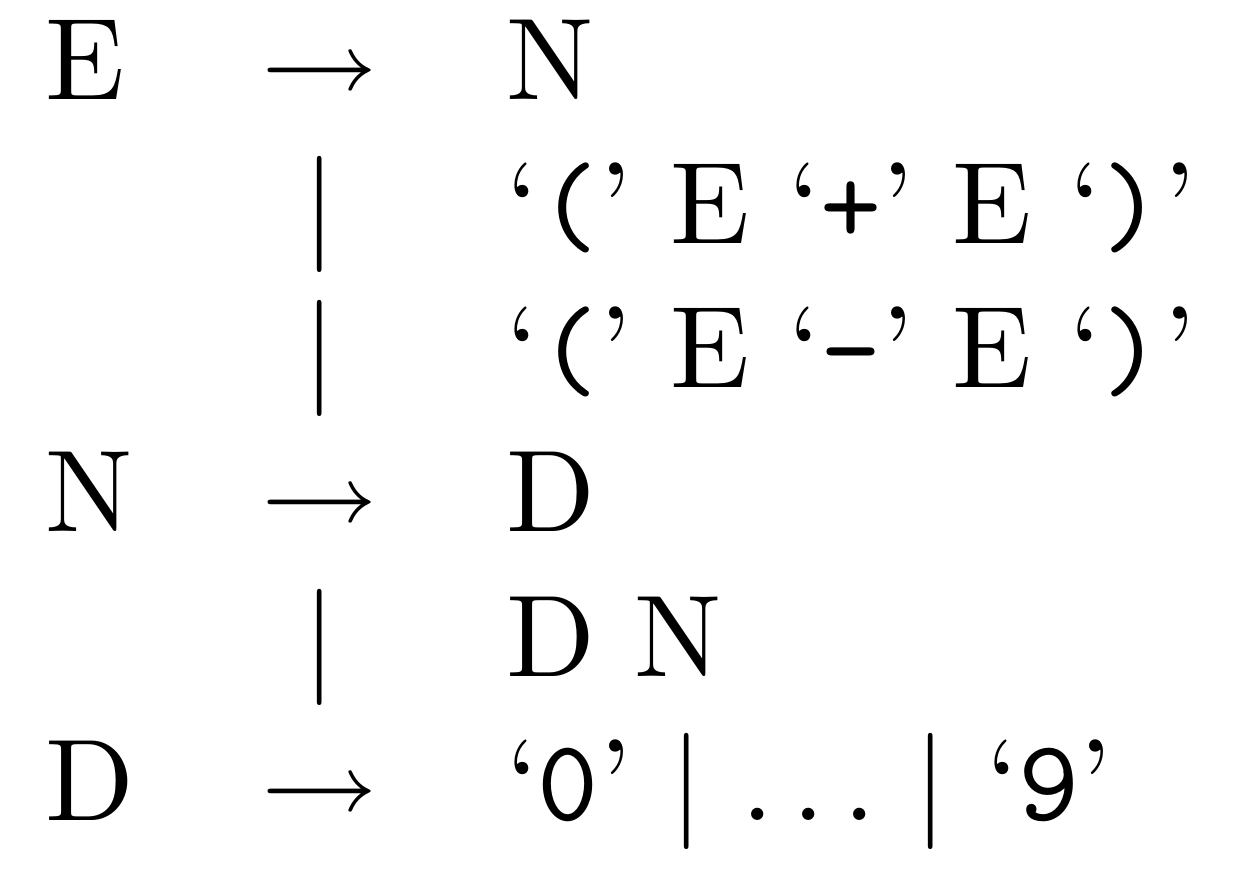
\includegraphics[width=0.3\textwidth]{pics/cfg_example}
    \caption{Μία CFG για μία απλή αριθμητική γλώσσα}
    \label{fig:cfg_example}
\end{figure}

Το Σχήμα \ref{fig:peg_example} παρουσιάζει την αντίστοιχη PEG.

\begin{figure}[h]
    \centering
    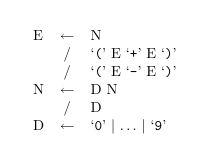
\includegraphics[width=0.3\textwidth]{pics/peg_example}
    \caption{Μία PEG για μία απλή αριθμητική γλώσσα}
    \label{fig:peg_example}
\end{figure}

Πρακτικά, η περιγραφή της γραμματικής μας ορίζει νοηματικά τί θα έκανε ένας καθοδικός συντακτικός αναλυτής για να αναγνωρίσει μία συμβολοσειρά στην είσοδο.

Το Σχήμα \ref{fig:peg_parse_example} απεικονίζει πώς η συμβολοσειρά `$(12-3)$' μπορεί να αναγνωριστεί σύμφωνα με τη γραμματική στο Σχήμα \ref{fig:peg_example} \cite{Ford2002a}.

\begin{figure}[h]
    \centering
    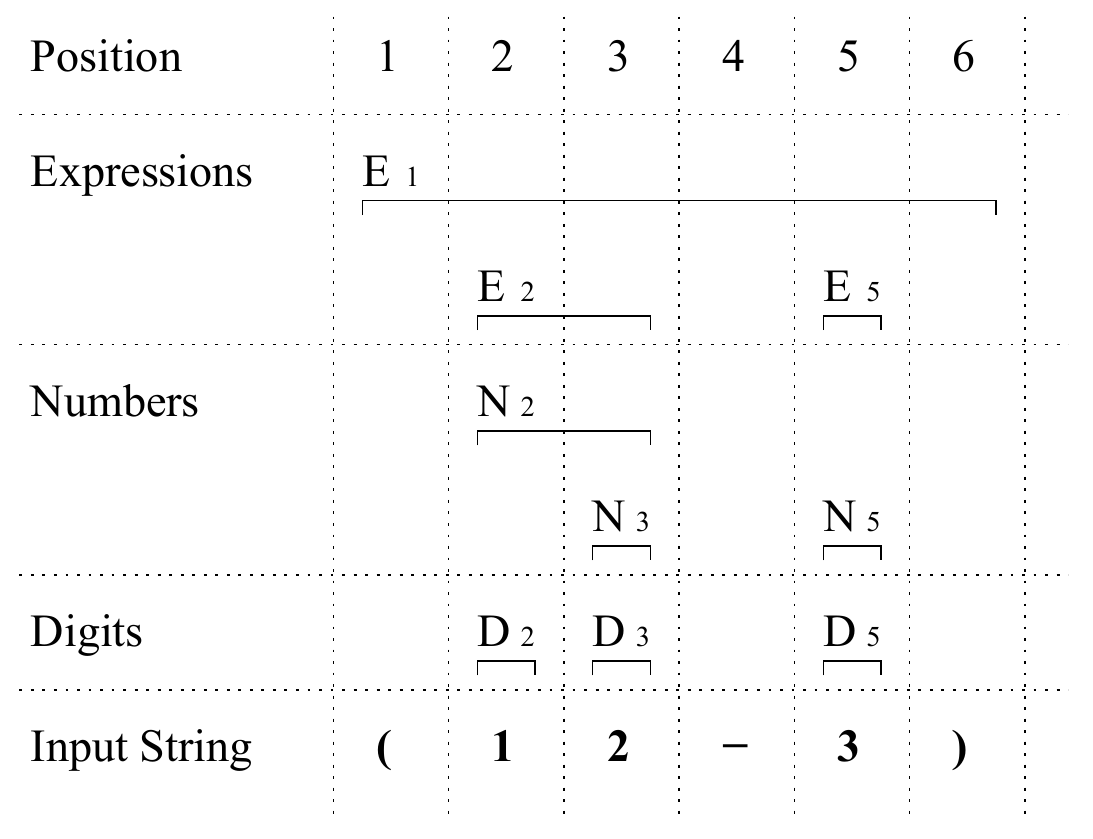
\includegraphics[width=0.5\textwidth]{pics/peg_parse_example}
	\caption{Αναγνωρίζοντας το `$(12-3)$' με βάση τη γραμματική στο Σχήμα \ref{fig:peg_example}}
    \label{fig:peg_parse_example}
\end{figure}

Ξεκινάμε προσπαθώντας να διαβάσουμε μία έκφραση $(E)$, από την αρχή της συμβολοσειράς.
Με βάση τον ορισμό της γραμματικής, για να αναγνωρίσει το μη τερματικό $E$, ο συντακτικός αναλυτής θα προσπαθούσε πρώτα να αναγνωρίσει την έκφραση $N$ που είναι η πρώτη εναλλακτική, οπότε προσπαθούμε και για τις δύο εναλλακτικές του $N$. Ωστόσο αποτυγχάνουμε καθώς στην είσοδο ο πρώτος χαρακτήρας είναι το '$($' και όχι κάποιο ψηφίο. 
Ακολούθως, πηγαίνουμε στη δεύτερη εναλλακτική για το $E$, τον κανόνα της πρόσθεσης εκφράσεων. 
Αυτός αναγνωρίζεται επιτυχώς με την αριστερή παρένθεση και μας καθοδηγεί στο να διαβάσουμε μία (υπο-)έκφραση ξεκινώντας στη θέση 2 της εισόδου.
Για να διαβάσουμε αυτή την υποέκφραση επιχειρούμε ξανά την $N$ εναλλακτική.
Πλέον, η πρώτη εναλλακτική του $N$ επιτυγχάνει, διαβάζοντας ένα ψηφίο στη θέση 2, και αναδρομικά ελέγχει για ένα ψηφίο στη θέση 3. 
Η πρώτη εναλλακτική του $N$ (δηλαδή η $D N$) αποτυγχάνει γιατί το ψηφίο στη θέση 3 δεν ακολουθείται από άλλα ψηφία, ωστόσο η δεύτερη εναλλακτική ($D$) επιτυγχάνει να αναγνωρίσει το ψηφίο, οπότε παράγει το αποτέλεσμα $N_3$ στο σχήμα. 
Η επιτυχημένη προσπάθεια καθιστά επιτυχημένη την αναγνώριση του $N$ στη θέση 2, οπότε το $N$ πλέον έχει ως αποτέλεσμα δύο κολλητούς χαρακτήρες, δηλαδή το $N_2$.
Αυτό οδηγεί στην έκφραση $E_2$ στο σχήμα. 
Επιστρέφοντας στο διάβασμα μίας έκφρασης στη θέση 1, η δεύτερη εναλλακτική αποτυγχάνει διότι η έκφραση $E_2$ ακολουθείται από ένα '$-$' αντί από ένα '$+$'.
Όμως, αν χρησιμοποιήσουμε την τρίτη εναλλακτική του $E$, αυτή επιτυγχάνει αφού αναγνωρίζει την αριστερή παρένθεση και την $E_2$ όπως και πριν, ενώ τώρα πετυχαίνει το '$-$', το ψηφίο $E_5$ στη θέση 5, και τη δεξιά παρένθεση. 
Επομένως, η έκφραση $E_1$ γεννιέται που αναγνωρίζει όλη τη συμβολοσειρά εισόδου.

\section{Άπληστη και Μη Ντετερμινιστική επανάληψη}
Ο κανόνας για το μη τερματικό $N$ δείχνει μία από τις πιο σημαντικές διαφορές μεταξύ των PEGs και των CFG γραμμτατικών.
Στη γραμματική του Σχήματος \ref{fig:cfg_example} η σειρά των δύο εναλλακτικών για το μη τερματικό δεν έχει σημασία, επειδή η επιλογή είναι μη ντετερμινιστική και προσανατολισμένη στο να γράφονται συμβολοσειρές και όχι να διαβάζονται.
Στην PEG του Σχήματος \ref{fig:peg_example}, η σειρά με την οποία εξετάζονται οι εναλλακτικές έχει σημασία: αν επιλέγαμε τη συντομότερη εναλλακτική πρώτα ($D$), τότε η μακρύτερη εναλλακτική δεν θα χρησιμοποιούνταν ποτέ.
Το αποτέλεσμα θα ήταν μία γραμματική που δεν θα μπορούσε να αναγνωρίσει τη συμβολοσειρά `$(12-3)$' διότι η ανάλυση του μη τερματικού στη θέση 2 θα κατανάλωνε μόνο το `$1$' στον αριθμό $12$, αφήνοντας το `$2$' να το αναγνωρίσουν άλλοι κανόνες ξεκινώντας πάλι από τη θέση 1.

Εξαιτίας αυτής της διαφοράς, οι δομές με επανάληψη σε μία PEG είναι εκ των πραγμάτων περισσότερο "άπληστες" παρά μη ντετερμινιστικές: μια επαναληπτική δομή πάντα καταναλώνει όσο περισσότερο κείμενο μπορεί, ανεξάρτητα από τα συμφραζόμενα στα οποία βρίσκεται. 
Αν στο παράδειγμά μας θέλαμε ξεφορτωθούμε το μη τερματικό $N$, θα μπορούσαμε να αντικαταστήσουμε την πρώτη εναλλακτική του $E$ με το `$D+$'.
Το αποτέλεσμα θα ήταν ακριβώς το ίδιο, γι' αυτό και ο τελεστής $+$ ονομάζεται "άπληστη θετική επανάληψη".

\section{Συντακτική ανάλυση ολόκληρων συμβολοσειρών}
Αν η γραμματική στο \ref{fig:peg_example} χρησιμοποιηθεί για να διαβάσει τη συμβολοσειρά `$(12-3)XYZ$', με αρχικό σύμβολο το $E$, τότε το αποτέλεσμα θα είναι "επιτυχία", ωστόσο μόνο το `$(12-3)$' θα έχει καταναλωθεί, αφήνοντας το `$XYZ$' ως υπόλοιπο. 
Όταν η πρόθεσή μας είναι να αναλύσουμε συντακτικά μία συμβολοσειρά, συνήθως θέλουμε να το κάνουμε μέχρι τέλους, και όχι μόνο σε ένα τμήμα της.
Ευτυχώς, η συμπεριφορά αυτή είναι εύκολο να υλοποιηθεί προσθέτοντας ένα νέο αρχικό σύμβολο $S$ όπως φαίνεται στο Σχήμα \ref{fig:whole_input}.

\begin{figure}[h]
    \centering
	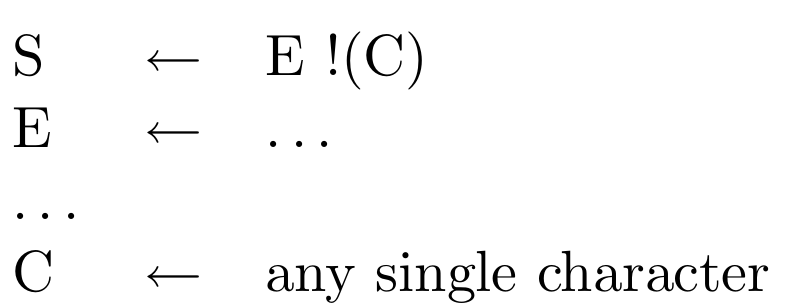
\includegraphics[width=0.35\textwidth]{pics/whole_input}
	\caption{Επέκταση της γραμματικής ώστε να εξετάζει όλη την είσοδο μέχρι τέλους}
    \label{fig:whole_input}
\end{figure}

Το αρχικό σύμβολο ψάχνει για μία έκφραση $E$, και μετά χρησιμοποιεί τον τελεστή "δεν-ακολουθείται-από" για να διασφαλίσει ότι τίποτα δεν έπεται μετά την αναγνωρισμένη έκφραση στην είσοδο.
Αν υπάρχει επιπλέον κείμενο που ακολουθεί την έκφραση, τότε το $C$ θα επιτύχει, κάνοντας το $S$ να αποτύχει. Αλλιώς, το $C$ αποτυγχάνει και το $S$ επιτυγχάνει.

Το $C$ σε αυτό το παράδειγμα είναι ένα μη τερματικό που αναπαριστά την \textit{κλάση χαρακτήρων}.

\section{Αριστερή Αναδρομή}

Σε μία γραμματική χωρίς συμφραζόμενα, τόσο η \textit{αριστερή} όσο και η \textit{δεξιά} αναδρομή επιτρέπονται. 
Ένα αριστερά αναδρομικό μη τερματικό έχει την ιδιότητα, αφού αναπτυχθεί μία ή περισσότερες φορές, να δίνει συμβολοσειρές η οποίες ξεκινούν με αυτό το μη τερματικό. 
Ομοίως, ένα δεξιά αναδρομικό μη τερματικό έχει την ιδιότητα να αναπτύσσεται σε συμβολοσειρές που \textit{τελειώνουν} με αυτό. 
Για παράδειγμα, είναι σύνηθες να εκφράζουμε τη σύνταξη αριστερά προσεταιριστικών τελεστών στα πλαίσια αριστερά αναδρομικών CFGs, και δεξιά προσεταιριστικούς τελεστές στα πλαίσια δεξιά αναδρομικών CFGs:

\begin{figure}[h]
    \centering
	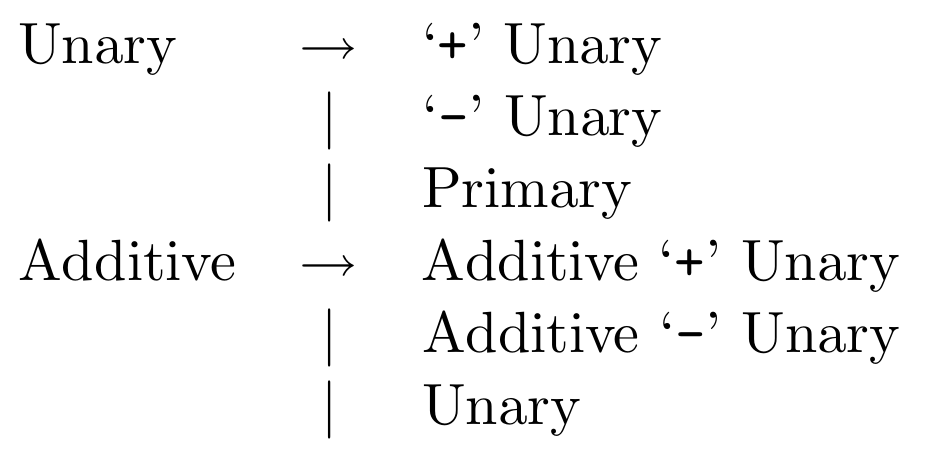
\includegraphics[width=0.40\textwidth]{pics/left_recursion}
	\caption{Αριστερά και δεξιά προσεταιριστικοί τελεστές σε μία CFG}
    \label{fig:left_recursion}
\end{figure}

Σε μία CFG ο δεξιά αναδρομικός ορισμός του $Unary$ υλοποιεί τους δεξιά προσεταιριστικούς μοναδιαίους τελεστές `$+$' και `$-$'.
Ομοίως, το $Additive$ υλοποιεί τους αριστερά προσεταιριστικούς τελεστές `$+$' και `$-$'.
Σε μία PEG, ενώ η δεξιά αναδρομή δουλεύει παρόμοια με τις CFGs, η αριστερή αναδρομή είναι εξ ορισμού λαθεμένη, καθώς η ερμηνεία της οδηγεί σε μία εκφυλισμένη αυτο-αναφορά. 
Για παράδειγμα, αν πάμε να εφαρμόσουμε αυτολεξεί τον κανόνα $Additive$ στα πλαίσια μίας PEG, τότε η ερμηνεία θα ήταν η εξής:
"Για να διαβάσεις μία $Additive$ έκφραση, πρώτα προσπάθησε να διαβάσεις μία $Additive$ έκφραση κ.ό.κ".

Σε μία CFG η αριστερή αναδρομή μπορεί να είναι βολική, ωστόσο δεν είναι απαραίτητη, καθώς οποιαδηποτε CFG που περιλαμβάνει αριστερή αναδρομή, μπορεί να γραφτεί σε μία ισοδύναμη CFG χωρίς αριστερή αναδρομή \cite{Moore2000}. 
Στις PEGs, συνήθως είναι πιο βολικό και ακριβές να χρησιμοποιούνται οι τελεστές `$*$' και `$+$', αντί της αριστερής ή της δεξιάς αναδρομής. 
Για παράδειγμα, η CFG του Σχήματος \ref{fig:left_recursion} μπορεί να γραφεί σε PEG ως:

\begin{figure}[h]
    \centering
	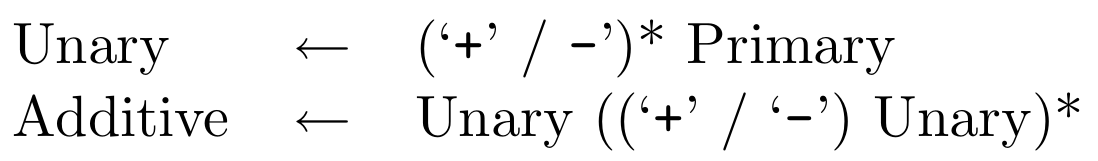
\includegraphics[width=0.45\textwidth]{pics/left_recursion_fix}
	\caption{Ισοδύναμη PEG χωρίς αριστερή αναδρομή}
    \label{fig:left_recursion_fix}
\end{figure}

Πάντως, αν είναι απαραίτητο, οι συντακτικοί αναλυτές των PEGs (τους οποίους θα περιγράψουμε παρακάτω), μπορούν να τροποποιηθούν ώστε να υποστηρίζουν αριστερή αναδρομή \cite{Warth2008}.


